\documentclass{scu-thesis}
% \usepackage{graphicx}	% for including graphics
% \usepackage{amsmath}	% for advanced typesetting of mathematics
% \usepackage{txfonts}	% for using the Times-Roman font
% \usepackage{natbib}	% for better citation styles
\usepackage{txfonts}
\usepackage{graphicx}
\usepackage{setspace}
\usepackage{indentfirst}
%\doublespace

% These must be set first ... the rest of the thesis commands rely on them.

\author{Kory Bartlett}
\author{Farzad Fred Feyzi}
\title{Shot Clock}
\department{Department of Computer Engineering}
\degree{Bachelor of Science in Computer Science and Engineering}


% Only bachelor's theses should have multiple authors and/or be from
% multiple departments.  Signatures required:
%
% Bachelor's theses: advisor(s), department chair(s)
% Master's theses: advisor, reader, department chair
% Doctoral theses: doctoral committee (including advisor), department chair

\begin{document}
\frontmatter
\signature{Thesis Advisor}
\signature{Department Chair}

\maketitle
\begin{abstract}
%A good abstract is a concise summary (1--2 paragraphs) of the entire
%project: introduction, problem statement, work accomplished, results,
%conclusions, and recommendations. When you write the abstract, imagine
%that the reader will not read anything else, but that you must get
%your major point across immediately. This requires efficiency of words
%and phrases. An abstract is written to stand alone, without jargon or
%eference to figures and tables in the report body.
\doublespacing
\par The sports sector has experienced major growth over the past couple of decades and is anticipated to grow even faster in the foreseeable future, especially as media technology continues to advance and access to sports games continues to increase. As the audience of sports enthusiast and observers expands, more people may miss the most recent and interesting sporting events from the previous night. Many websites have attempted to serve these groups, but they have become cluttered with articles or short-clips that hold little to no significance to the sporting outcome. These websites have begun  to get away from the simple need of highlighting an event in an efficient format. Our solution, Shot Clock, is a simple, centralized web application to view sports highlights that functions by taking advantage of today's modern technologies. The web application will also provide a user experience that promotes simplicity, continuity, and ease of use when navigating the application. Users will also have the opportunity to create custom lists so that they can be kept up to date to their favorite teams. Succeeding in these major facets will provide audiences with the practicality of easy access to precise replays delivering an innovative experience that users will appreciate.

\end{abstract}


\tableofcontents
\listoffigures

\mainmatter
\chapter{Introduction}

\section{Motivation}
\par The sports industry in North America alone currently is worth 60.5 billion dollars and this industry has been projected to grow to 73.5 billion dollars by 2019. This rise in projected growth happens due to the fact that media companies are making larger deals, which in turn is caused by more people being entertained by sports. However, not everyone can make it to the television for every game, and not everyone has the time to watch a full-length game. This creates the need for easy access to fast sports highlights and other sports statistics that can help individuals relive the exciting moments in a match/game without having to spend too much of their time watching the actual event. Therefore, a user should be able to navigate to a website and within a few seconds be watching the game he or she intended to watch. Quite a few of these websites currently exist today, but we think that they could be dramatically improved.
\par There are many websites today that have attempted to solve this issue, but while attempting to cover all sports related issues, they have gotten away from the simple goal of highlighting sports in a precise fashion. Websites like ESPN.com, FoxSports.com, and BleacherReport.com all encompass some of the highlights from a particular sport’s league, but they all have become cluttered with loosely related sports articles and irrelevant game interviews. The current methods include too many articles that often take up too much space within a user’s window. This is troublesome because the user should simply get to the video highlights in a fast manner, without having to traverse the entire cluttered site for over 30 seconds; the search time must be decreased. In addition to that, when it comes to different sports, the current implementation does not have any continuity between the sports; in other words, the view for soccer typically varies significantly from the view for basketball. Website usability is key for user experience because discontinuity between key pages can lead to frustrations causing a user to discontinue use of a website. Lastly, many current implementations do not have a reliable source of efficient highlights. For example, some websites will leave out certain games within a league, creating an inconvenience for the user who is just trying to view his or her desired highlight.

\section{Solution}
\par Our solution is to use modern technologies in order to create a simple, centralized web application in which users can easily view any highlight within any sport and league. We will make sure there is continuity between different sports pages by using a one-size fit all view. In addition to that, there will be unique customization features, so highlights can be catered to users’ interests. The system will pull videos and gifs with thorough content ensuring fans can experience a full game in a matter of minutes, and we can will guarantee no game within a season is missing. The window for viewing video will be conveniently placed in the middle of the website, making it easier for people to see, with navigation bars around that centralized feature. We will not include articles because that takes away from the viewing experience and makes it harder to search for highlights in a timely manner. Overall, the different, more simple user experience along with more unique customization and guaranteed highlights will provide users who are interested in highlights the ideal platform for them to follow their teams and games. 

\chapter{Requirements}

\section{Introduction}
	Requirements define and qualify what the system needs to do. Functional requirements specifically define what must be done and what the solution must do. Non-functional requirements have to do more with performance and reliability and thus, talk about how the functional requirements need to be achieved. Lastly, design constraints constrain the solution rather than the problem.
\section{Functional Requirement}
	\begin{itemize}
    \item Critical
    	\begin{itemize}
        \item The system will allow the user to search for videos
        \item The system will allow the user to see a steady stream of videos
        \item The system will allow the user to add videos to his video queue 
    	\end{itemize}
   	\item Recommended
    	\begin{itemize}
		\item The system will give the user the ability to sign in and sign out 
        \item The system will allow the user to customize his or her settings in order to create a more personalized web app
        \item The system will not allow for repeat username
    	\end{itemize} 
    \end{itemize}
\section{Non-Functional Requirement}
	\begin{itemize}
    \item Critical 
    	\begin{itemize}
    	\item The system will be put together using user friendly UI 
        \item The system will be  easy to  navigate 
        \item The system video portal will be consistently laid out between pages
        \item The system will be extensible to work for varying sports leagues        
    	\end{itemize}
    \item Recommended
    	\begin{itemize}
        \item The system will be secure and have a well tested sign in process 
        \item The system will be responsive 
    	\end{itemize}
	\end{itemize}
\section{Design Constraints}
	\begin{itemize}
    \item Critical
    	\begin{itemize}
    	\item The system must be web based 
    	\end{itemize}
	\item Suggested
    	\begin{itemize}
        \item CSS frameworks and other modern libraries should be used because of its ability to create good looking UI 
        \item Sport themed images and icons are encouraged in order to go with the theme of the project 
    	\end{itemize}
	\end{itemize}
\chapter{Use Cases}

\section{Introduction}
This section describes the four to five main use cases that a student can perform. The first subsection contains a diagram displaying the main user and the user's four to five possible actions. The second subsection details the name, goal, conditions, and steps corresponding to each use case. 

\section{Diagrams}
\begin{figure}[!ht]
      \centering
      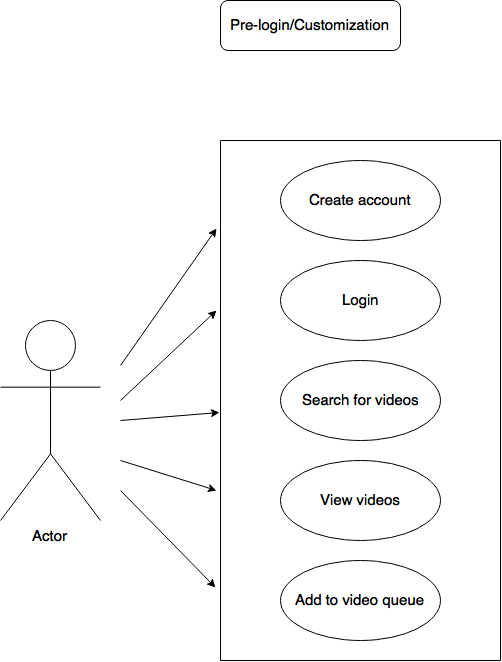
\includegraphics[width=0.5\textwidth]{useCasePreLogin}
      \caption{Use Case Diagram of Pre-login}	
\end{figure}
\begin{figure}[!ht]
      \centering
      \includegraphics[width=0.5\textwidth]{useCasePostLogin}
      \caption{Use Case Diagram of Post-login}	
\end{figure}


\section{Use Case Description}
\begin{itemize}
\item Create account
	\begin{itemize}
	\item Name: Create an account to be used on website
    \item Goal: To create an account ti be used on website
    \item Actor: User
    \item Preconditions
		\begin{enumerate}
		\item User must be on webpage
        \end{enumerate}
    \item Steps
    	\begin{enumerate}
		\item User selects my settings
        \item User selects create an account 
        \item User enters desired username and password combination
        \item User submits username and login combination to system to be submitted
        \end{enumerate}
    \item Post-conditions
		\begin{enumerate}
		\item Assuming user's username is unique, the combination gets committed to the system
        \item The website loads user's stored data and allows for user customization 
        \item The website returns to the overall view of the website with user now logged-in
        \end{enumerate}
    \item Exceptions
    	\begin{enumerate} 
    	\item User's username needs to be unique so process may need to be repeated to achieve a unique result, user will be alerted of error occurring 
        \end{enumerate}
    \end{itemize}

\item Login
	\begin{itemize}
	\item Name: Login to website
    \item Goal: To sign in to website
    \item Actor: User
    \item Preconditions
		\begin{enumerate}
		\item User must be on webpage
        \item User must have a preexisting account
        \end{enumerate}
    \item Steps
    	\begin{enumerate}
		\item User selects my settings
        \item User can create an account to be used to login
        \item User enters login credentials
        \item User submits login to be signed into website
        \end{enumerate}
    \item Post-conditions
		\begin{enumerate}
		\item User's username is checked if it exists in the system
        \item The matching username and password are returned 
        \item The user's password is then checked against the returned username's password
        \item Assuming the credentials match, the user is then logged on to the system
        \end{enumerate}
    \item Exceptions
    	\begin{enumerate} 
    	\item User who has entered information but has not created an account will be asked to create an account
        \end{enumerate}
    \end{itemize}
    
\item Search for Videos
	\begin{itemize}
	\item Name: Search for videos 
    \item Goal: Allows user to specify videos to watch
    \item Actor: User
    \item Preconditions
		\begin{enumerate}
		\item User must be entered into system
        \end{enumerate}
    \item Steps
    	\begin{enumerate}
		\item User types into textbox to specify which sports video to view
        \item User video returned ready to view
        \end{enumerate}
    \item Post-conditions
    	\begin{enumerate}
		\item User continues on website to view video
        \end{enumerate}
    \item Exceptions
    	\begin{enumerate}
    	\item Video requested by the user is unavailable in database of video sources, so user is alerted of unavailability of video and can re-enter search items to perform another search
    	\end{enumerate}
    \end{itemize}

\item View Videos
	\begin{itemize}
	\item Name: View videos 
    \item Goal: To watch video on website
    \item Actor: User
    \item Preconditions
		\begin{enumerate}
		\item User must be entered into system
        \item User must allow video to play
        \end{enumerate}
    \item Steps
    	\begin{enumerate}
		\item User able to enjoy video playback
        \end{enumerate}
    \item Post-conditions N/a
    \item Exceptions N/A
    \end{itemize}
    
\item Add to Video Queue
	\begin{itemize}
	\item Name: Add videos to queue
    \item Goal: To use website to add user specific videos to queue
    \item Actor: User
    \item Preconditions
		\begin{enumerate}
		\item User must be entered into system
        \item User must have already searched for videos
        \end{enumerate}
    \item Steps
    	\begin{enumerate}
		\item User types into textbox to specify which sports video to view
        \item Video is added to the back of the queue
        \item Video is ready to be viewed in queue order
        \end{enumerate}
    \item Post-conditions
    	\begin{enumerate}
		\item To view video user must allow video to play through
        \end{enumerate}
    \item Exceptions
    	\begin{enumerate}
    	\item If the user has cleared their queue of videos after the new video is added to the queue then the recently added video along with other videos queued for viewing will be removed from queue. System will play the newest video added next
    	\end{enumerate}
    \end{itemize}
    
\item Customize Settings
	\begin{itemize}
	\item Name: Customize settings
    \item Goal: To customize personal settings
    \item Actor: User
    \item Preconditions
		\begin{enumerate}
		\item User must be entered into system
        \item User must have an account and be logged into system
        \end{enumerate}
    \item Steps
    	\begin{enumerate}
		\item User clicks my settings tab
        \item User can edit their username and password
        \end{enumerate}
    \item Post-conditions
    	\begin{enumerate}
		\item User must save changes made when editing their profile
        \end{enumerate}
    \item Exceptions
    	\item *unable to udpate*
    \end{itemize}
    
\item View Customized Videos
	\begin{itemize}
	\item Name: View customized videos 
    \item Goal: To view list of customized videos referred to as MyReplay
    \item Actor: User
    \item Preconditions
		\begin{enumerate}
		\item User must be entered into system
        \item User must be logged into system
       	\item User must have edited and saved their MyReplay preferences
        \end{enumerate}
    \item Steps
    	\begin{enumerate}
		\item User returns back to home page of website
        \item User can enjoy video playback of queue
        \end{enumerate}
    \item Post-conditions
    	\begin{enumerate}
		\item The program grabs the desired data entries
        \item Videos will play in most recent found from database
        \end{enumerate}
    \item Exceptions
    	\begin{enumerate}
    	\item User may watch an old video if the update has not been run by program
    	\end{enumerate}
    \end{itemize}
    
\item Sign Out
	\begin{itemize}
	\item Name: Sign out of website
    \item Goal: To sign out the users profile from the website
    \item Actor: User
    \item Preconditions
		\begin{enumerate}
		\item User must be entered into system
        \item User must be signed in to the system
        \end{enumerate}
    \item Steps
    	\begin{enumerate}
		\item User clicks my settings tab
        \item User clicks log off button
        \item User profile has exited the system
        \end{enumerate}
    \item Post-conditions
    	\begin{enumerate}
		\item Clear user data from the website
        \item Reset the website so it functions as if a new user has just entered 
        \end{enumerate}
    \item Exceptions N/A
    \end{itemize}
    
\end{itemize}
\chapter{Activity Diagram}

\section{Introduction}
This activity diagram outlines the basic flow of user activity while using the our webpage. Users, upon entering the site, can choose to sign-in to their accounts for customization or continue to the site without features of customization. The user can then search for specific videos to view. If the user decides to not search for a specific video then they will view the queue of videos available.\newpage
\section{Diagram}
\begin{figure}[!ht]
      \centering
      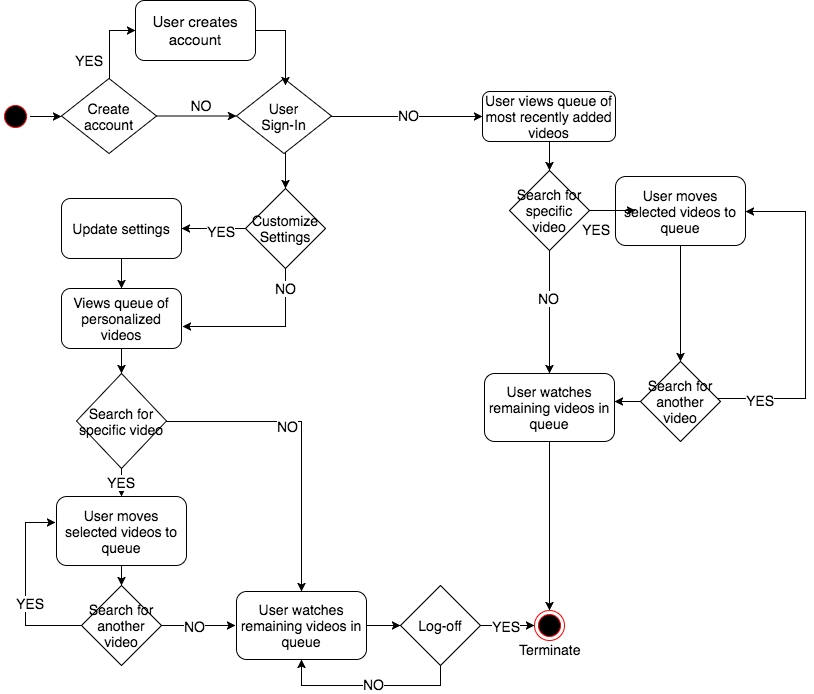
\includegraphics[width=\textwidth]{activityDiagram}
      \caption{Activity Diagram}	
\end{figure}
\chapter{Conceptual Model}

\section{Introduction}
	The conceptual model illustrates through mock ups how the system will appear to different actors who might use the system. The webpage will look the same overall, however it has small differences between users who decide to create an account and users who don’t have an account.  Figure 5.1 shows the overall view. This remains the same for both users and it is what a user sees from a cold start. Figure 5.2 shows the user login and registration page. Figure 5.3 shows the user customization page. Here a user can select the teams he or she is interested in. Figure 5.4 shows what the screen looks like after a user has logged in.

\section{Landing Page}
\begin{figure}[!ht]
      \centering
      \fbox {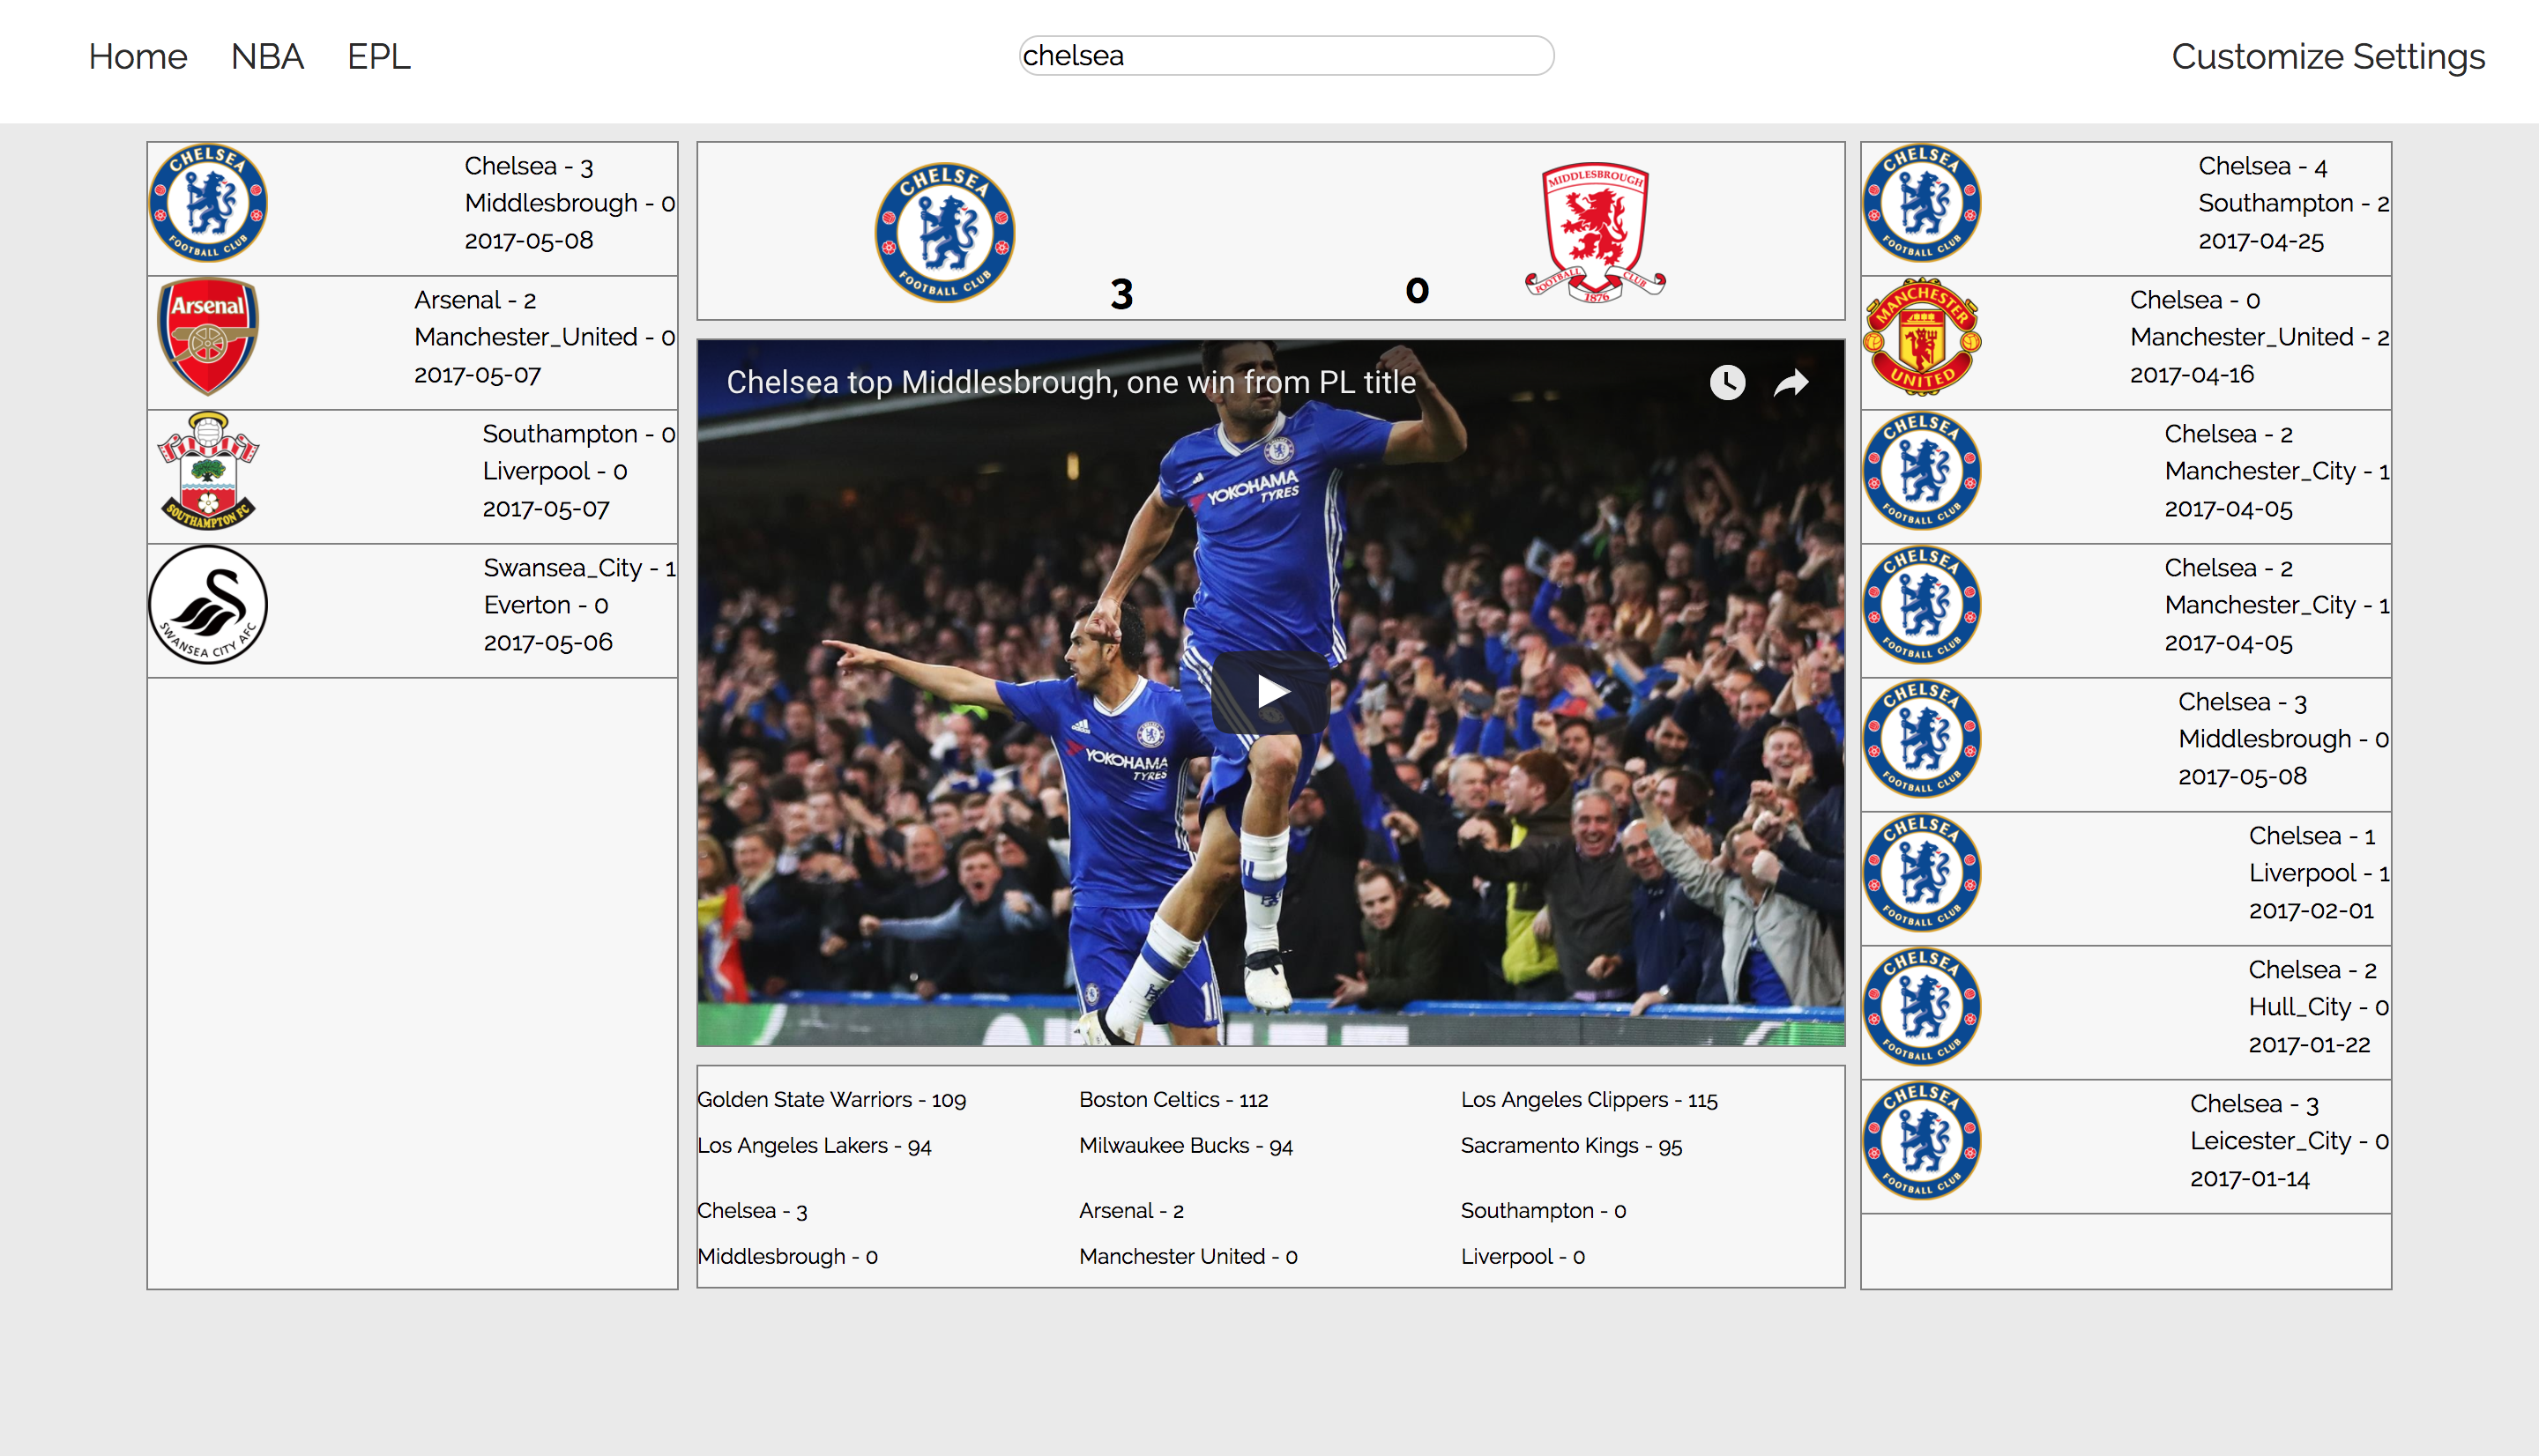
\includegraphics[scale=0.25]{landing.png}}
      \caption{Overall view of website as guest}	
\end{figure}

\section{User Login/Registration Page}
\begin{figure}[!ht]
      \centering
      \fbox {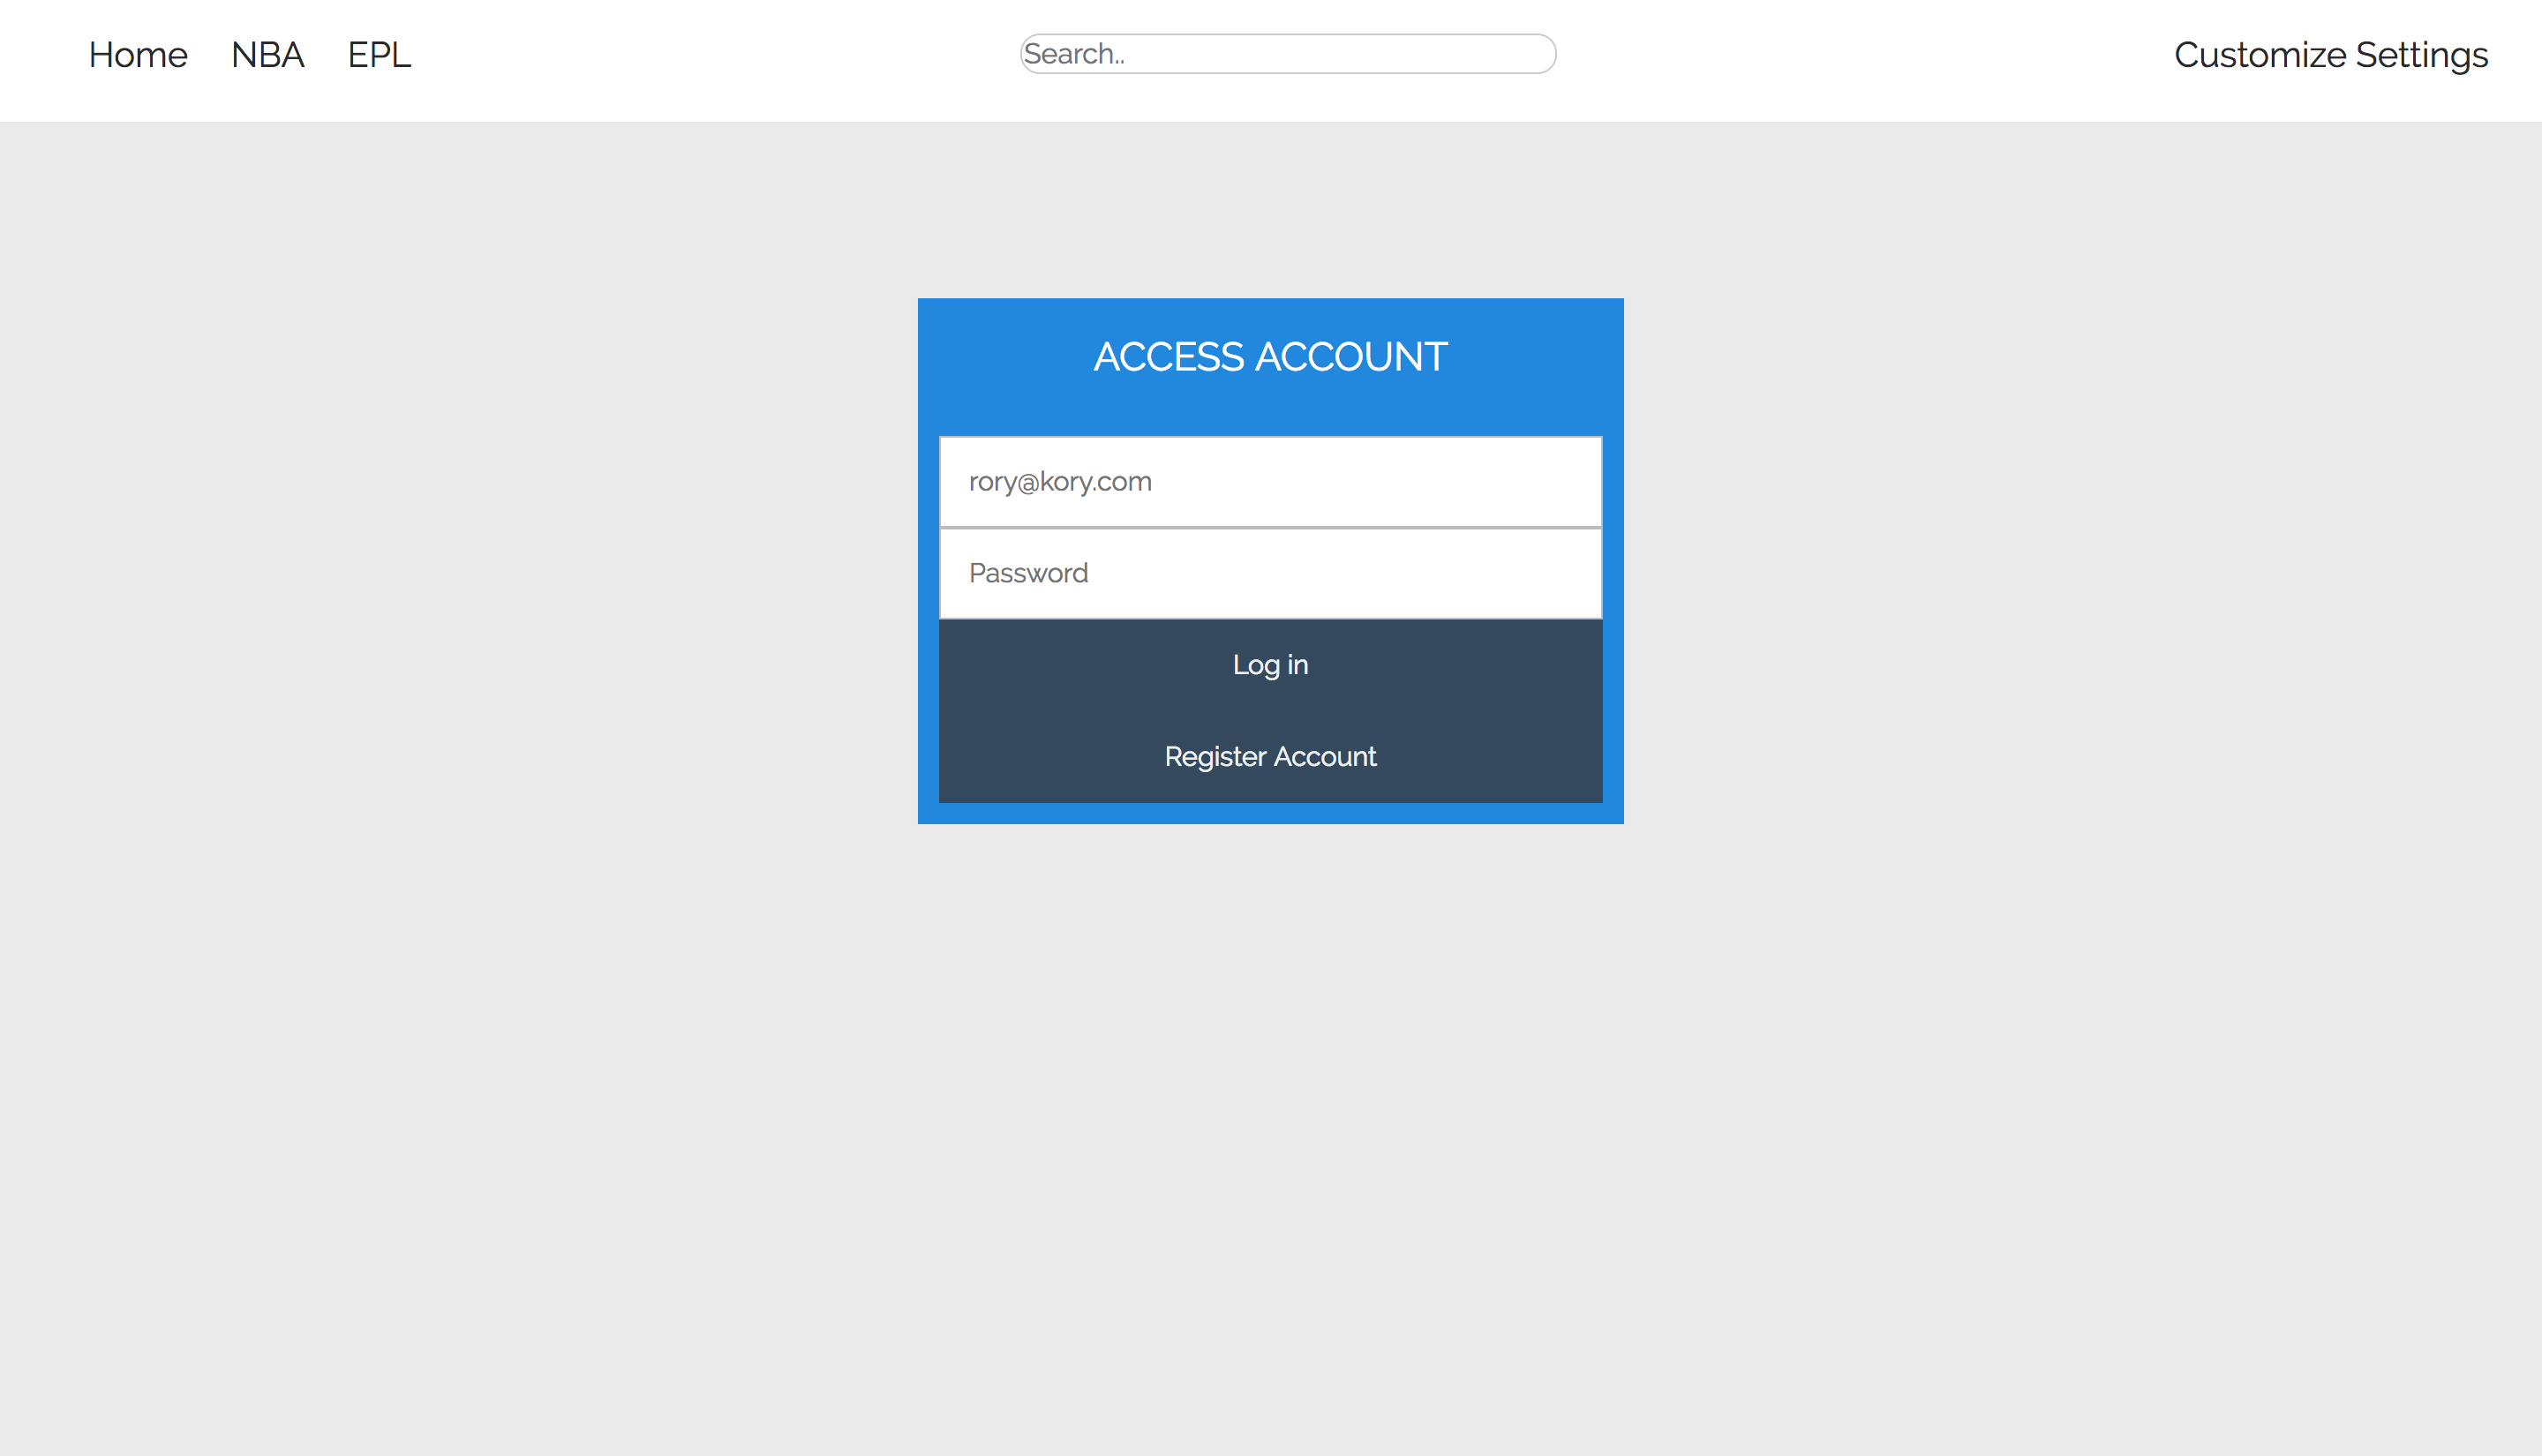
\includegraphics[scale=0.25]{signin.png}}
      \caption{Account creation}	
\end{figure}

\section{User Customization Page}
\begin{figure}[!ht]
      \centering
      \fbox {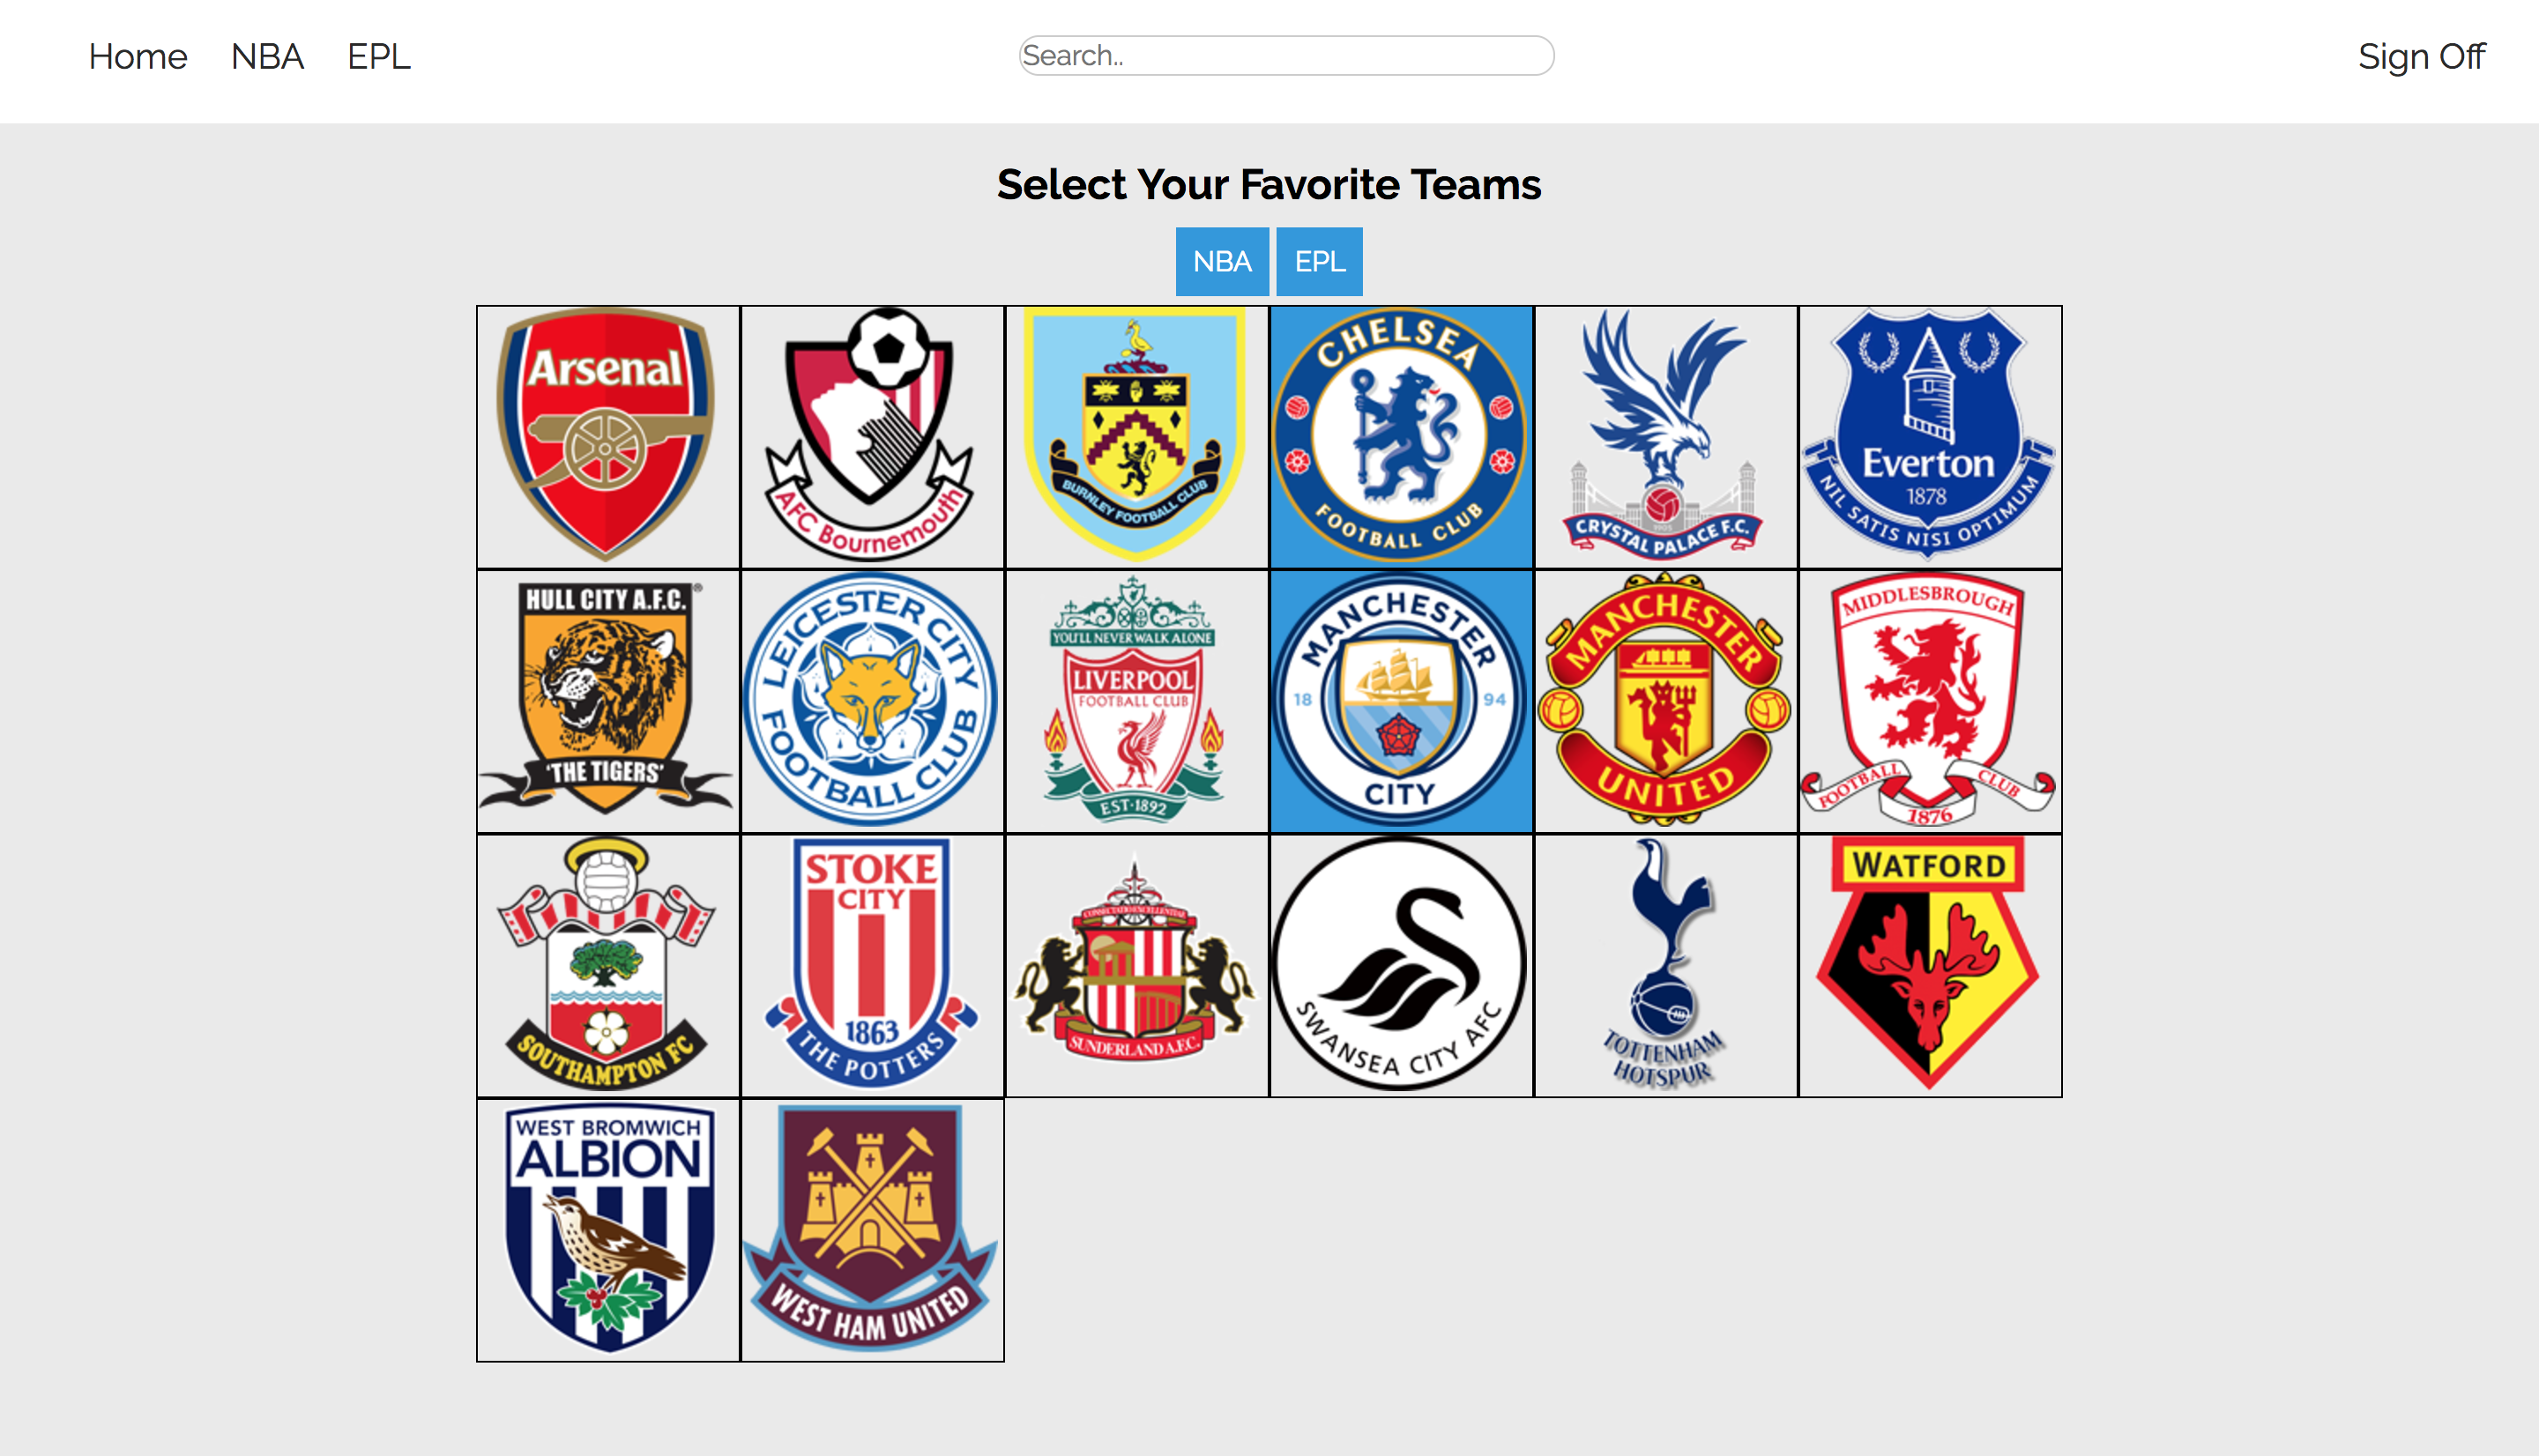
\includegraphics[scale=0.25]{register.png}}
      \caption{User customization of favorite EPL soccer teams}	
\end{figure}

\newpage
\section{Logged-In User Page}
\begin{figure}[!ht]
      \centering
      \fbox {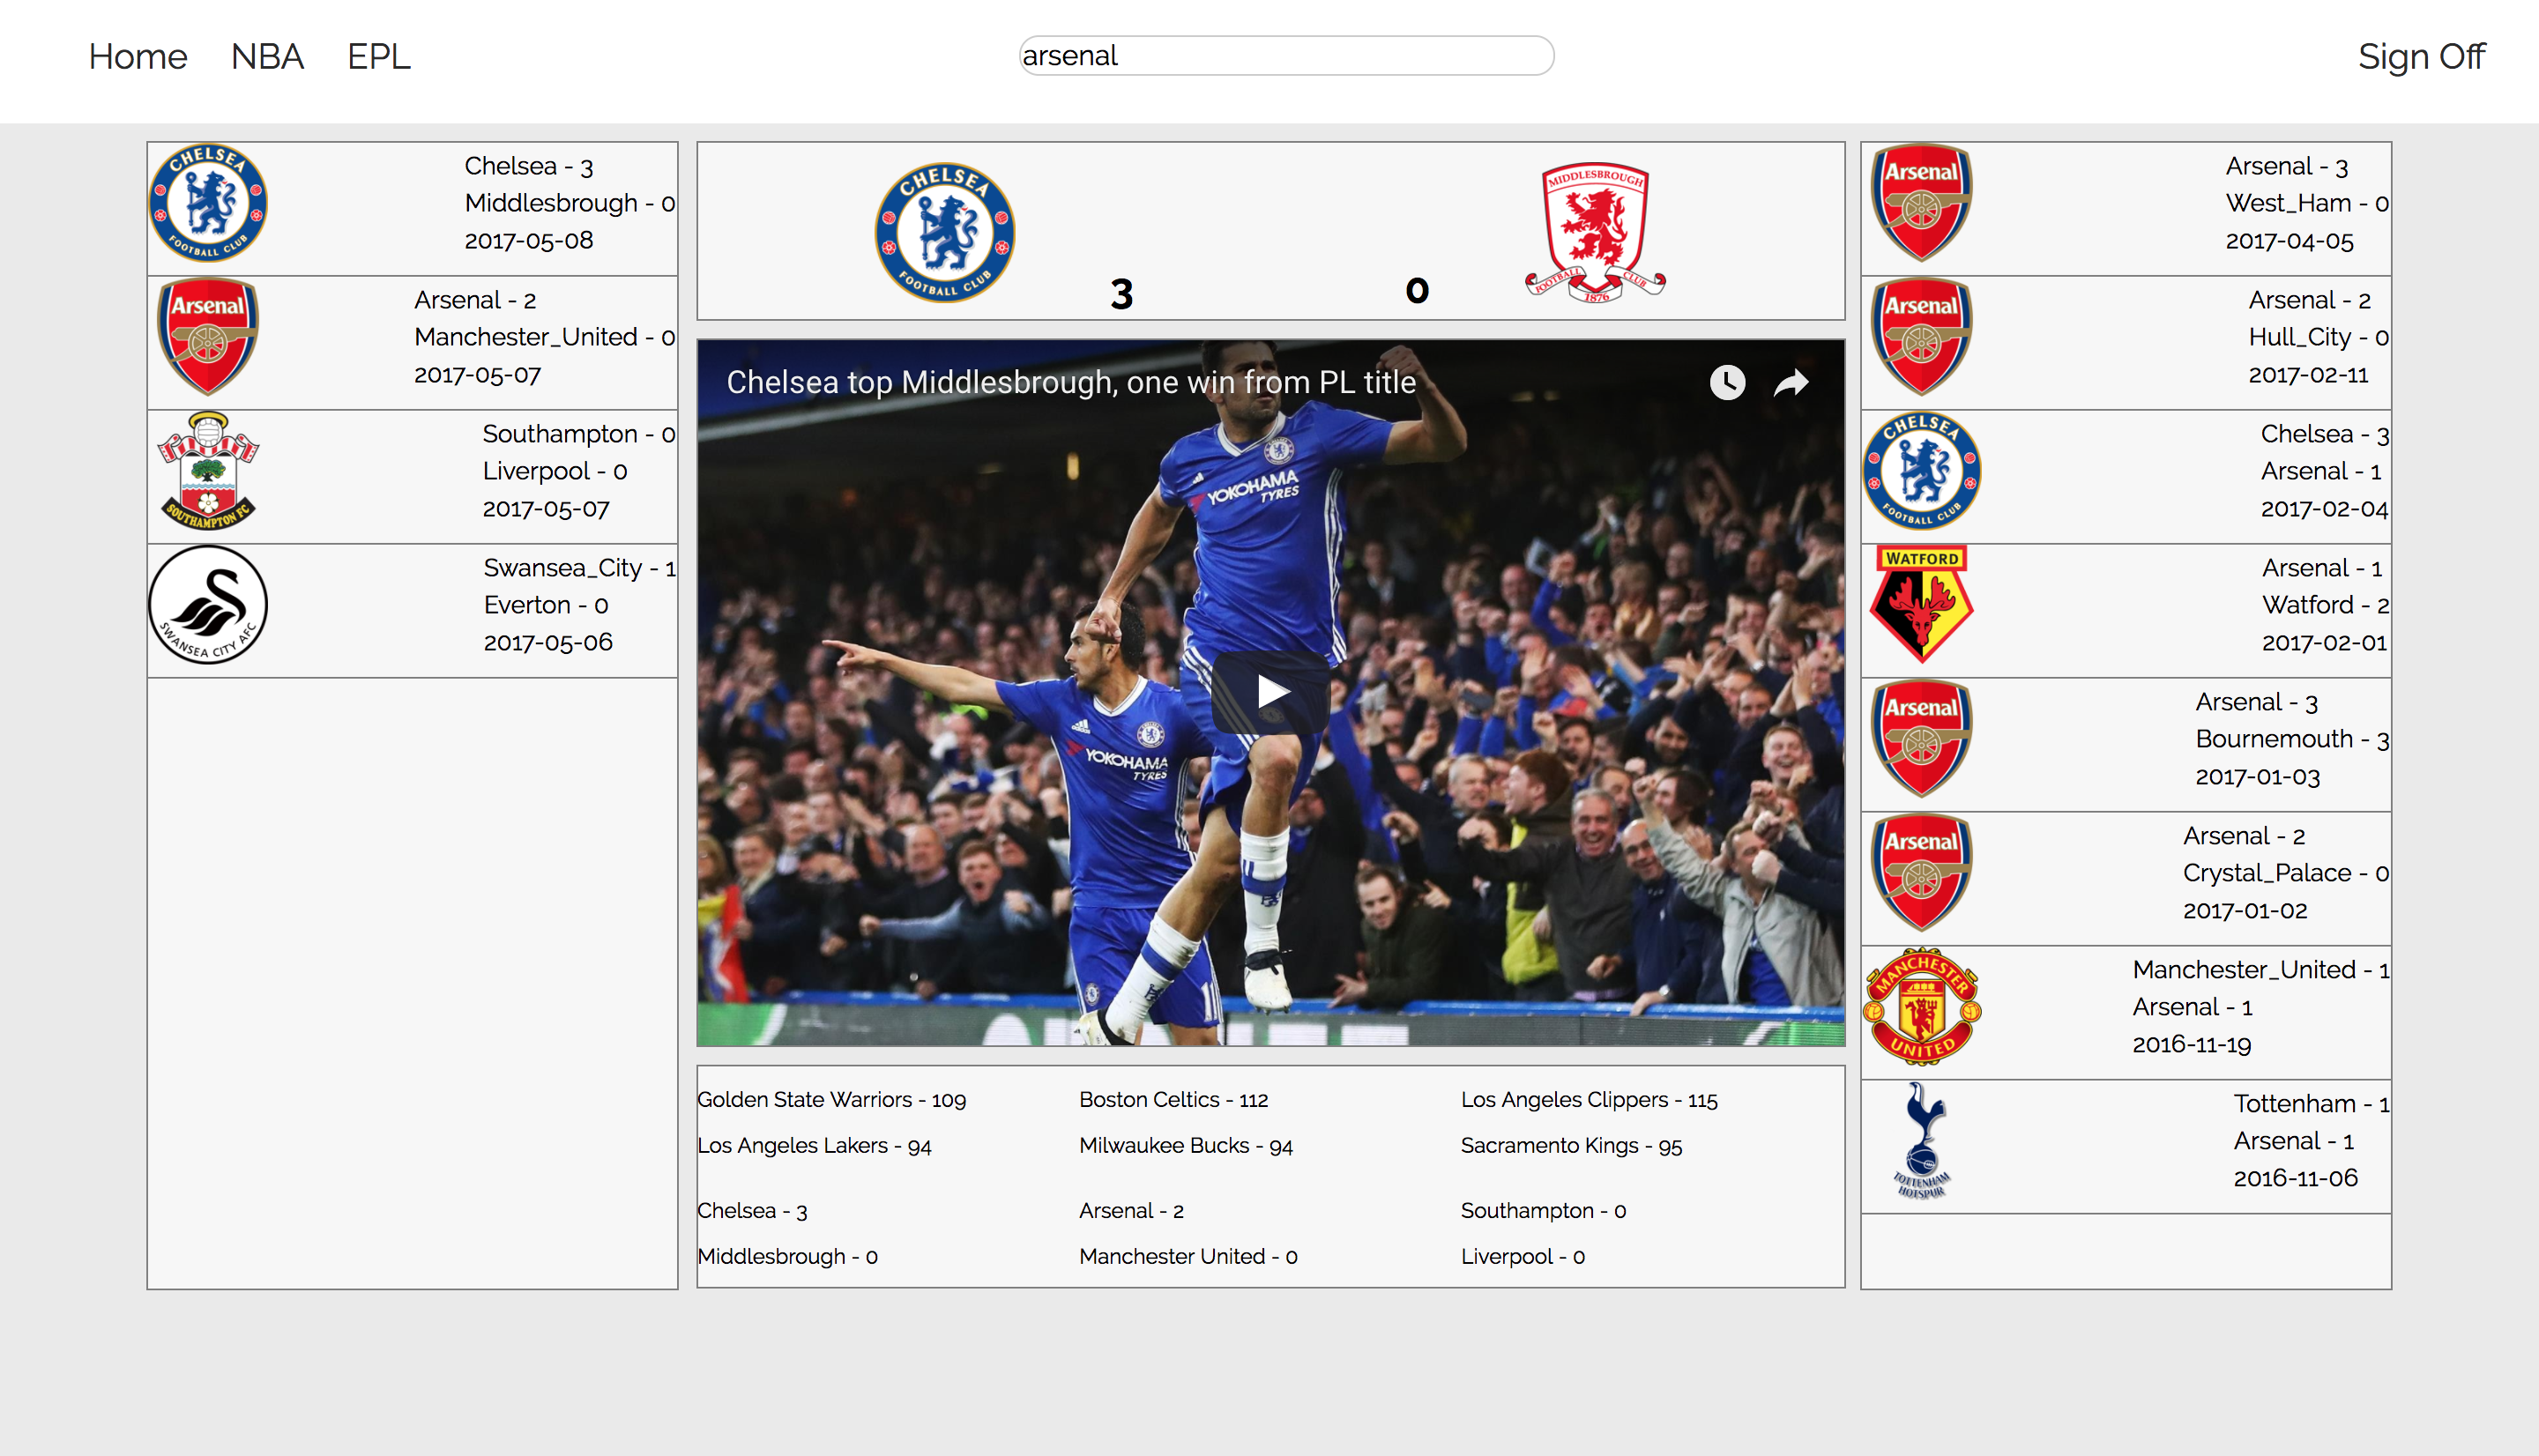
\includegraphics[scale=0.25]{loggedin.png}}
      \caption{Logged-In user on homepage}	
\end{figure}
\chapter{Technologies Used}
The technologies used outlines the current technologies and languages used to complete the project. These technologies were chosen because of their ability to provide the services needed to complete the requirements. These technologies are listed below:
\begin{itemize}
	\item Ajax - Added to help make data population and page loading asynchronous
	\item CSS - Front end language to help style the web application solution
	\item ElasticSearch - An open-source, easily scalable search engine based on Lucene that serves to hold and index data
	\item Express JS  - A specific framework within Node that helps out with route handling and middleware creations
	\item Firebase - Google backed suite that provides a real-time database and login configuration system
	\item HTML - Front end language used to serve as the structure for the website solution
	\item JavaScript - Programming language used for both the front and back end 
	\item Kibana - Data visualization technology that is easily integrated with the Elasticsearch index
    \item Materialize CSS - A front end library provided by Google for styling purposes
	\item Node JS - The back end language used to help connect the server with our ElasticSearch instance and the running server to handle the web crawler and event handlers	
\end{itemize}

\chapter{Architectural Diagram}
\section{Introduction}
	The Architecture Diagram illustrates the kind of software architecture used to create the system. An architecture allows the way the system functions to be easily understood. Our application’s system uses a client-server architecture, illustrated in the figure below.
\section{Diagram}
\begin{figure}[!ht]
      \centering
      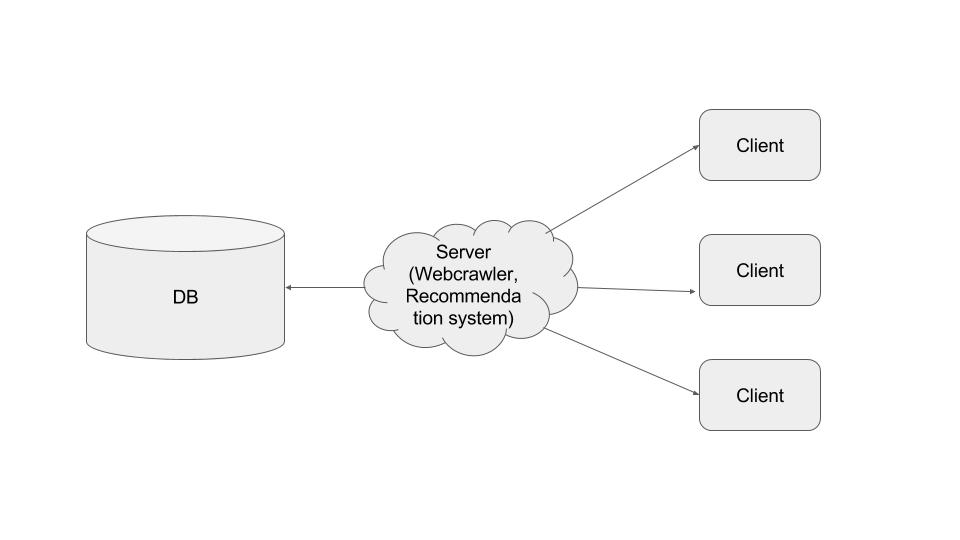
\includegraphics[width=\textwidth]{architecturalDiagram}
      \caption{Architectural Diagram}	
\end{figure}
\section{Architectural Rationale}
	As stated above, our solution uses the client-server architecture. Users, or clients, can access the application through its url. The server then does a lot of the event handling. The server is responsible for having a running web crawler on a cron job that will seek to obtain data, and then index the data appropriately in our real time ElasticSearch database. The server will also be handling the recommendation system as well, so users can have the data they’re customized data. The server will then connect to the database to store the links to the videos ( so we don’t need to actually store massive files). The database will have easily indexable data. 
\chapter{Design Rationale}

\section{Introduction}
	The design rationale gives reasons for the decisions we made in the design of the product. This primarily justifies the choices made about the user interface design and the technologies used.
    
\section{User Interface Design}
	The user interface for this application will have the look and feel of a single page application (SPA), but will consist of numerous pages; thus, requiring numerous routes. We chose this because we want to account for continuity among pages, but also prioritizing the viewing experience. Except for having to make changes to his or her account, the user should always be able to have a running video feed on the application. Having an interface as such will keep the user busy watching, while being able to do numerous other tasks (like searching for videos) at the same time. 

\section{Technologies Used}
	The technologies used are basic, yet modern web technologies and frameworks that should render similar pages across multiple browsers. We will use an ElasticSearch instance along with a MongoDB database to enable easy indexing of data and application model creation. We will use an Amazon EC2 instance to gain flexibility and ease in our deployment process. We are using technologies that our development team is familiar with to ensure a short and doable development timeline. Node JS along with the powerful Express JS framework will be used to keep a running server as well organize our routes to different pages. This will also be especially helpful when we make many HTTP requests to GET or POST data. We chose to use the Materialize CSS framework because it makes the styling fairly easy and responsive, and Angular JS to guide in that effort as well. We reserve the right to not use Materialize CSS however, should it make creating responsive elements harder. In that event, we will resort to simply using CSS media queries. 
\chapter{Test Plan}

\section{Unit Testing}
\par Unit testing of our web application was useful in the preliminary stages of testing. This form of testing can be done to ensure that we have correct functionality of individual features as well as catch any bugs related to the features. The first focus, and most important, of our testing was to carefully develop our web page to reflect our wire frame concepts. With an active web page, we were able to ensure that our website dimensions held up adequately on different browsers and varying computer operating systems. Testing our web page on varying platforms ensured the integrity of our aesthetics was kept amongst the possible user base. Another focus of this testing was to ensure our web crawler grabs the correct data we specified. The web crawler testing was tedious, but necessary, as we had to carefully prepare it for the possible items it needed to search for on-line. We were able to notice that some games were initially missed because team names were abbreviated from time to time. After adjusting the web crawler to accommodate these occurrences it was able to work successfully in grabbing the designated videos. The next function we addressed was the logging in and registration of user profiles to create a profile to use on our web page. Creating and connecting several user accounts to the firebase system allowed us to test for successful users registrations as well as logins. These tests verified that we had a user system properly set up and accessible for future integration testing. Lastly, the elasticsearch database we decide to use was also tested to ensure it can hold a high amount data entries as well as be reliable to grab entries efficiently. Once all of our video information was carefully assembled we were able to push it into the database. We used Kibana as a visualizer as it showed the successful amounts of pushed entries into our database so we could catch early on if any items were not accounted for after the transfer of information. This was a fantastic tool as it revealed to us that some game scores and/or team names were not imported into the database, which we then quickly amended solving the issue. It also allowed us to test queries to our database which we used to discover the most optimal search terms to return the most relevant information to users. 

\section{Integration Testing}
\par The integration testing of our program was one of the most crucial steps. During this testing phase we began connecting services and functionality to ensure that the program can function as a whole. Components will be pieced together one at a time so that the errors can be pinpointed and the problem can be specified. As each service is connected to the completed system the errors will become obvious as to which portion of the project is improperly functioning. We first connected our web crawler to the database. We needed to ensure that the information we grabbed was following the schema needed to be imported into the database. Although the web crawler correctly grabbed information, we realized that when the information was temporarily stored, such as the date meta data, the formatting would be distorted and unusable to the database. Adjusting the date data string format and encapsulating all the information as a JSON object allowed for the two services to work together. Now that we had our information collection coupled with our database we were able to move forward into integration with our web page. The web page integration with the previous components was focused on connecting the elasticsearch database to the web page features. We needed to ensure that the user inputs would work with the database queries. After connecting the services we discovered that the user inputs needed to match our database entries, so depending on the user input we would modify their search terms to ensure the user would get the results they requested. Our final step for integration testing was linking our web application’s features to be used with user profiles. During this portion of testing we used user profiles to select their favorite teams to be saved to their account preferences. This integration of services revealed problems in saving user preferences to a profile if they had not selected a specific team in a sport. Since the user selection for that sport was empty the data entry would not be created in the database and thus no longer accessible in the future. We were able to address this issue with a dummy variable so that the user could adjust their preferences appropriately later on.  


\section{Alpha Testing}
\par Alpha testing was completed in-house by our team once integration testing was completed. During alpha testing we were able to check that the core functionality of the product was near completion and fully functional now that all components were connected. As the system was tested, we were able to find the bugs that still persisted as well as the errors that were still prevalent in the code causing erroneous results. Initially the elasticsearch and web page were able to run simultaneously, as expected. However, playing the videos had become an issue due to the CORS being sent accessed. This issue was only noticeable once all the features were combined and running together on the network. It was resolved after modifying the proper headers and locations of the files. Along with catching the bugs in the program, we will also be able to ensure that all requirements were properly addressed and satisfied by the system. In this step we were able to reexamine our requirements to address those we felt could be further developed in our project as we had established the initial abilities we could build upon of the project. 

\section{Beta Testing}
\par During beta testing we expanded testing from only group members to friends, colleagues, or others interested in the project. By this step most user cases were thoroughly tested and functional. We used tester feedback to improve the user-interface aspects that were generally agreed upon. A few areas repeatedly mentioned were adjusting which pages were linked to specific buttons and the queue lengths. An example of this was most of our testers were either basketball fans or knew more of the sports teams from that league. This influenced our decision to show basketball team's first when customizing user preferences. Users also suggested that we limit the initial queue size so that when they search for videos they can add a greater of number of videos to the queue after a search.  As some bugs will be still uncaught before this process, using beta testers will ensure that all possible situations and edge cases are exhausted so that the program is ready to be used. 

\chapter{Risk Analysis}

\section{Introduction}
This section describes the several possible risks associated with the project. The first subsection contains descriptions of the different columns in the Risk Analysis table. The second subsection contains the table itself, which lists details such as the numerous risks and their associated levels of severity and consequences. 

\section{Table Description}
\begin{itemize}
	\item Name of Risk: Specifically identifies specific risks associated with project.
    \item Consequences: The outcome of the risks if they occur.
    \item Probability: The likelihood of the risk occurring.
    \item Severity: The effect the risk can impose on the project.
    \item Impact: The probability multiplied by the severity. It determines a quantitative measurement of the risk on the project.
    \item Mitigation Strategies: Possible actions to take to prevent the risks from occurring.
\end{itemize}

\begin{figure}[!ht]
	\centering
    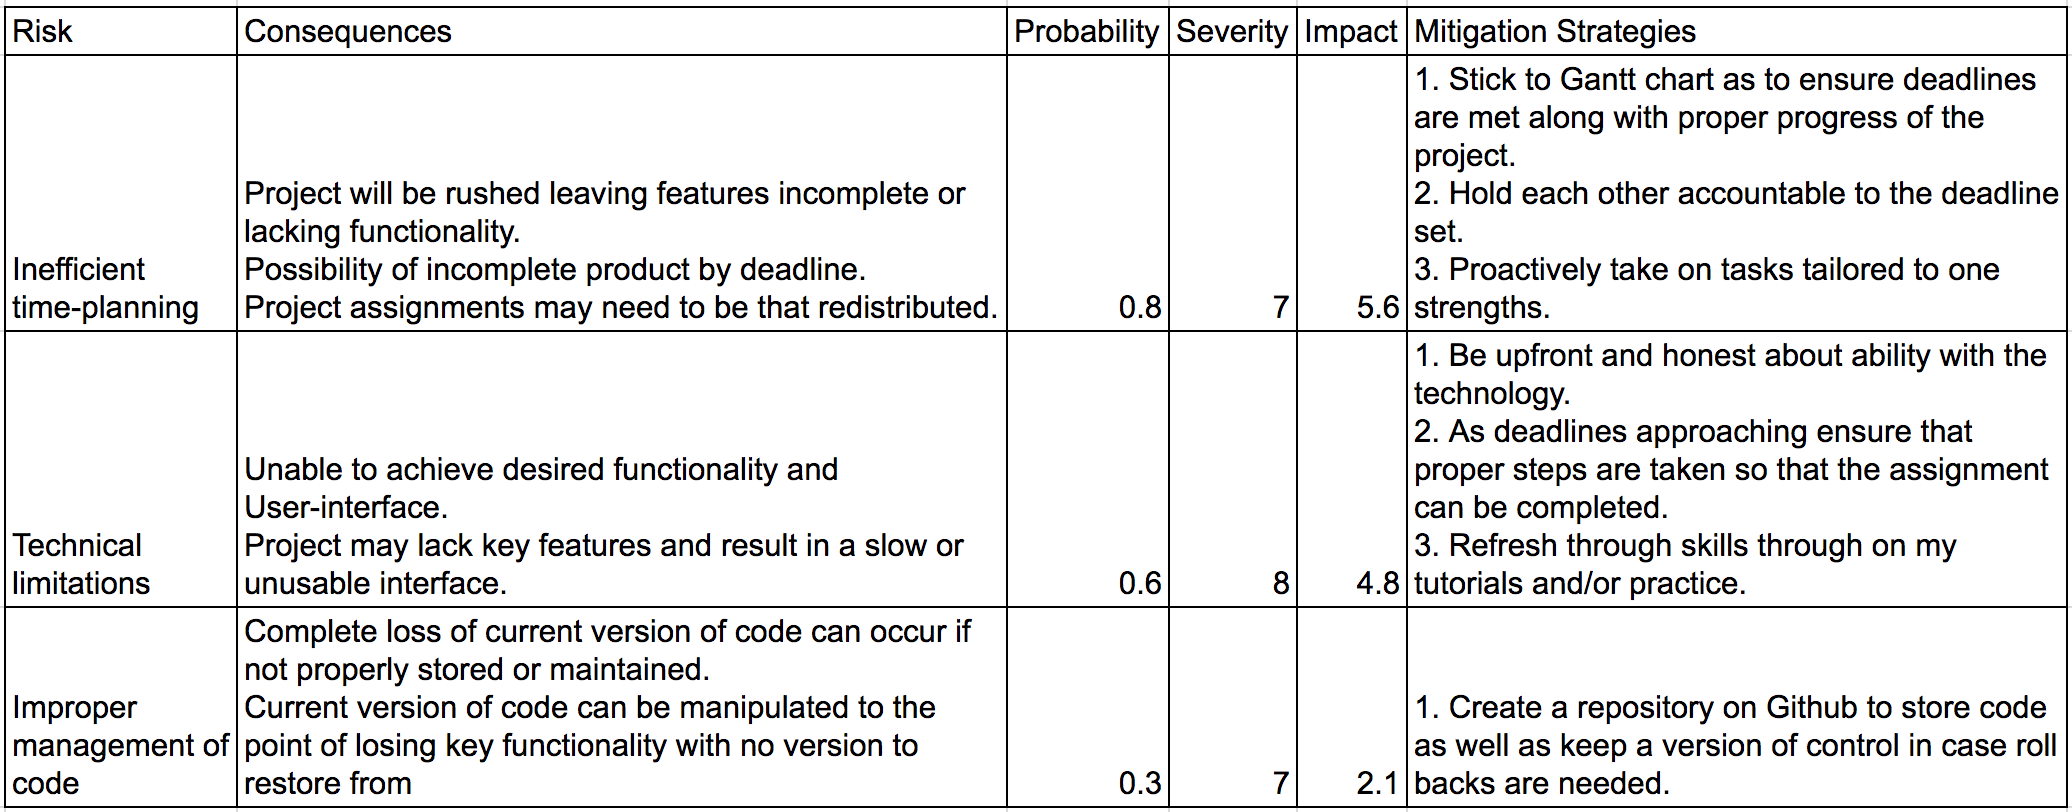
\includegraphics[angle=270,scale=0.6]{riskTable}
    \caption{Risk Analysis Table}
\end{figure}
\chapter{Developmental Timeline}

\section{Introduction}
This section covers our planned developmental timeline. We present our proposed plans via Gantt chart. The project was divided into major steps: project requirements, design, implementation, testing, and documentation. The tasks were dispersed on a per person basis. 

\begin{figure}[!ht]
	\centering
    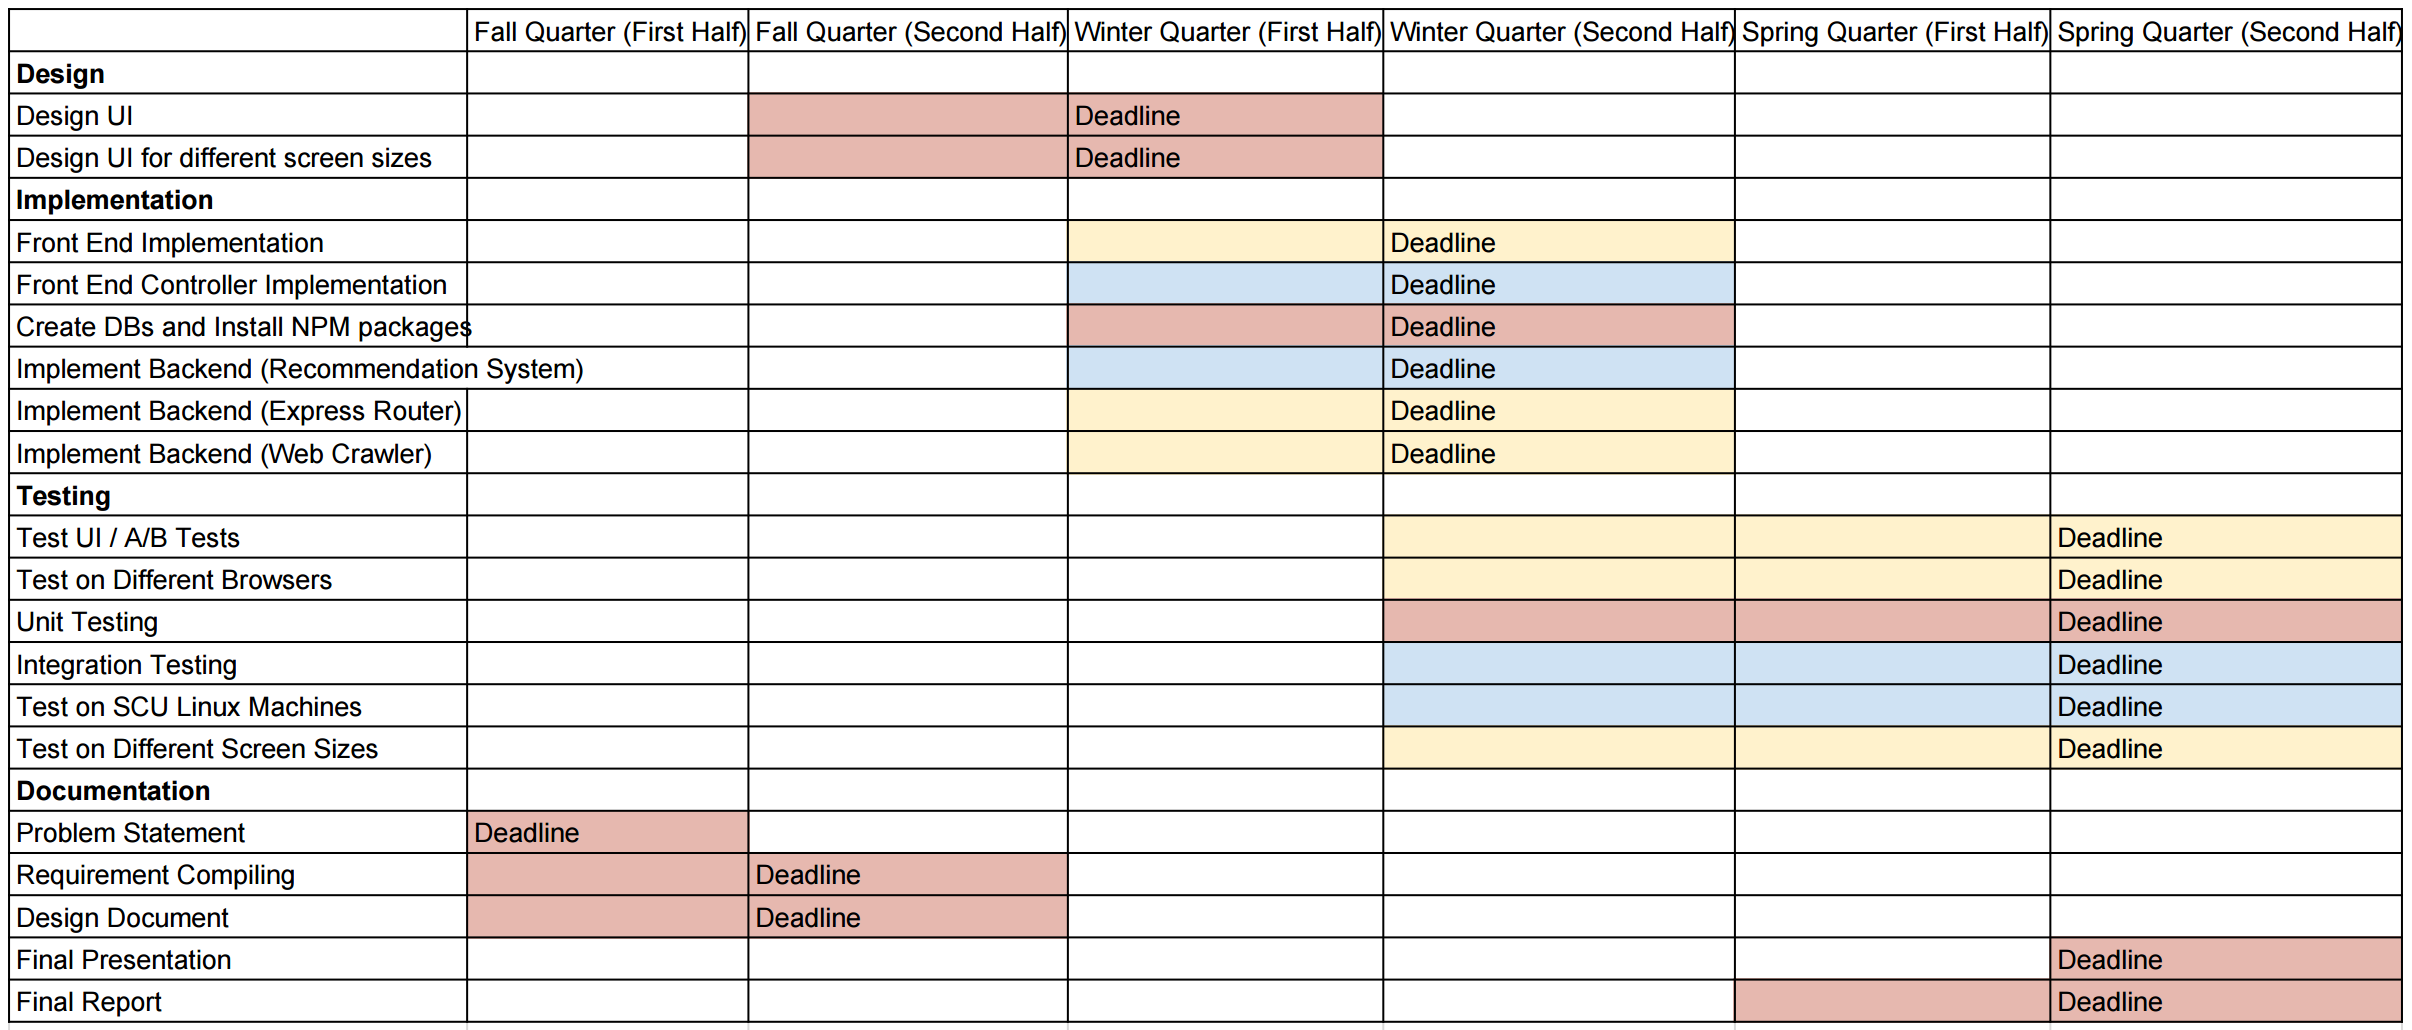
\includegraphics[angle=270,origin=c,width=.5\textwidth]{gantt}
    \caption{Gantt Chart}
\end{figure}
\chapter{Societal Issues}

\section{Introduction}
\par In any engineering project, there are many different social issues that could and should be taken into account. We initially knew some of the issues that we would encounter as we moved forward, and as we began to actually develop our project further and further, we thought of more and more issues that we needed to consider and take into account. 

\section{Ethical}
\par We faced a little bit of ethical dilemmas as we proceeded to work on our project. First and foremost, we recognized that since we needed to scrape videos off the internet and call different APIs, we had to make sure that the videos we used had a Creative Commons License. A Creative Commons license allowed us to legally share other people's’ work, in this case being the sports highlights clips. In addition to that, we were able to request  sports score data from a company known as MySportsFeeds, and someone from the company personally reached out to us, giving us free access to use their service and allowed us to display that data. In addition to that, since there were many moving components, we made sure to always keep our project as a free service. We thought it was morally wrong to use other people's work to make money for ourselves. Lastly, since we did have a login and customization feature, we had to make sure that our users data was kept safe, which is why we opted to go with Google’s Firebase system. The service automatically encrypted our users passwords; therefore, no one could simply gain access to that. Fortunately, our project wasn’t dealing with very sensitive data nor any technology that could directly harm a user’s life, so our ethical considerations were thus limited.

\section{Economic}
\par As this was a web based project our goals can be reached through construction and design of code, which is a free resource. Also, because we currently hold student titles and our goals are not for profit, most services are offered at free or greatly reduced prices. Therefore, the current costs of our project totaled nothing. However, if we continue to improve the project post-graduation we may need to examine the services as we scale up server space and/or have a need for higher performing equipment, which will see the charges begin to add up . (Add line on how creative commons allows us free use of stuff) 

\section{Usability}
\par One of the main problems we were trying to address while working on our project was to make the service more user friendly by creating more continuity among different sport pages throughout the site. In our opinion, we definitely achieved that. Now users don’t need to get used to many different screens. In addition to that, we strived to limit the number of buttons on our website as well as create a large video player in the middle of the screen to keep videos playing at all times. When it came to modifying settings, we went with a visual approach so that the user could clearly see what he or she is selecting. Lastly, our entire application was built in different modules, and this allows us to easily adjust the site to make it mobile and tablet friendly!

\section{Lifelong Learning}
\par For our project we decided to challenge ourselves by tackling the problem using modern frameworks and technologies. This project has inspired us both to pursue further projects to improve our proficiency and expertise regarding these technologies. Because these technologies are relatively new there are less references available so this improved our ability to digest the given documentation to debug and understand our issues better. This was an important skill to have gained and cemented into our repertoire because it can be applied later on in life on future projects and developments. 
\chapter{Conclusion}

\par Overall, while the project was long and arduous,  we made many mistakes along the way and we learned a lot as well. 

\par We were able to achieve our goal, in creating a web application that made viewing sports highlights a much simpler, more efficient, and user friendly experience. We were able to set up an instance with Elasticsearch, connect it to our Node server, launch the express JS framework, and visualize all the back end data on Kibana (all relatively new tools that we were able to learn along the way). We were able to work with Google’s Firebase, in order to create a user customization feature so that users can view videos that would be interesting to them. Most importantly, we were able to see out a project that looked delightful as a mock up and put it in production mode, launched as an Amazon EC2 instance. 

\par Along the way, many obstacles came our way, and we had to find ways to get around them. That being said, we were able to remember what they were, and learn from them in the future. First and foremost, we learned that we need to allocate more time for deployment purposes. When initially creating our Gantt Chart, we underestimated the time it would take to deploy both our ElasticSearch instance as well as our Node server. This led to a lot of unnecessary stress, and could have been avoided, had we allocated more time. Secondly, we learned that we needed to properly and more frequently push our code to the version control system. Sometimes we got caught in developing our own respective part of the project, and when we both pushed, there were a lot of merge errors. If we had pushed our code more frequently, this would have been avoided. Next, we learned that we need to use our technology stack to its full potential. Essentially, we set up an ExpressJS application; however, we found ourselves sometimes writing external JS files to do a mini task. This is not what Express was meant to do, and we believe the request payloads throughout our application could have been smaller should we have stuck to programming the “Express way”. Lastly, we learned that we should not over complicate the problem. Whereas ElasticSearch is a great modern tool to use, its use could have been avoided, for we really didn’t need an indexable search engine running in our back end. Something like SQL would have done the job as well in this application. 

\par We encountered many  cross origin resource sharing (CORS) errors when initially testing our application, and did not really understand what was going on. One thing that could have been done better is to truly understand what was going on under the hood, instead of finding ways around that. In addition to that, the application, in its current state, is not mobile responsive yet, and that could/should have been completed. Learning more about how Elasticsearch scales is also another thing that could have been done. Elasticsearch uses a lot of new terminology, like “shards”, “documents”, and “mappings”, and it's important to know those to understand how to scale fast, should a lot of users be on our application making requests. Lastly, we could have gotten rid of all our external public Javascript files, and embedded that in the ExpressJS routes. That would have decreased our request payload, and simplified a lot of the code. 

\par For the future, we need to make the application mobile responsive, clean up the code base, understand everything regarding cross origin resource sharing, and lastly, understand how to scale the Elasticsearch, should that be necessary. Overall, this project has been a blast, and we have both been exposed to many new technologies that we previously did not know. Throughout the process, we ran into some obstacles, but we’re happy to say we always found ways to get through and around them. 

\backmatter
\end{document}
